\section {Vergleich von AdaBoost und GBT mit anderen Modellen}
In diesem Kapitel werden die zwei vorgestellten Boosting Algorithmen AdaBoost und GBT mit anderen bekannten Vertretern von ML-Modellen verglichen werden. Die Ergebnisse und Grafiken basieren auf einer Studie von Randal \textcite{Olson2018}, welche 13 unterschiedliche Algorithmen auf 165 Datensätzen evaluiert. Das Ziel dieses Kapitels ist nicht nur eine einfache Leistungsanalyse, sondern soll auch eine Empfehlung für die Praxis geben.

\subsection{Auswahl und Leistung der Algorithmen}
Die von \textcite{Olson2018} untersuchten Algorithmen sind eine Reihe von Klassifikationsmethoden, wie unter anderem Naive Bayes Varianten, logistische Regression, Support Vector Machines. Darüber hinaus werden auch baumbasierte Algorithmen wie Random Forests und Extra Trees analysiert. 

\subsection{Auswahl der Datensätze}
Eine gute Auswahl der Datensätze ist entscheidend für eine aussagekräftige Bewertung. Insgesamt wurden 165 Datensätze aus dem Penn Machine Learning Benchmark (PMLB) ausgewählt. In dieser Sammlung sind viele Klassifikationsprobleme enthalten, die sowohl für die Öffentlichkeit verfügbar sind, als auch in einem einheitlichen Format dargstellt werden.
\newline
Bei der Auswahl wurde vor allem auf eine breite Abdeckung vieler Arten von Klassifikationsproblemen geachtet. Das bedeutet unterschiedliche Datengrößen, Anzahl der Attribute und Schwierigkeitsgrade. Ein großer Teil der Datensätze ist aus dem Bereich der Bioinformatik, jedoch nicht in einem Ausmaß, welches die Aussagekraft der Studie einschränken wurde. Diese breite Auswahl soll eine faire Leistungsbeurteilung ermöglichen, welche auch Stärken, Schwächen und daraus resultierende Anwendungsgebiete aufzeigt.

\subsection{Ergebnisse der Studie}
In \autoref{fig:avarage_ranking_comparison} schneidet GBT am besten ab mit einer durchschnittlichen Platzierung von ca. Platz 3. AdaBoost liegt in diesem Ranking im unteren Mittelfeld mit einer durchschnittlichen Platzierung von ca. Platz 8.
\begin{figure}[H]
    \centering
    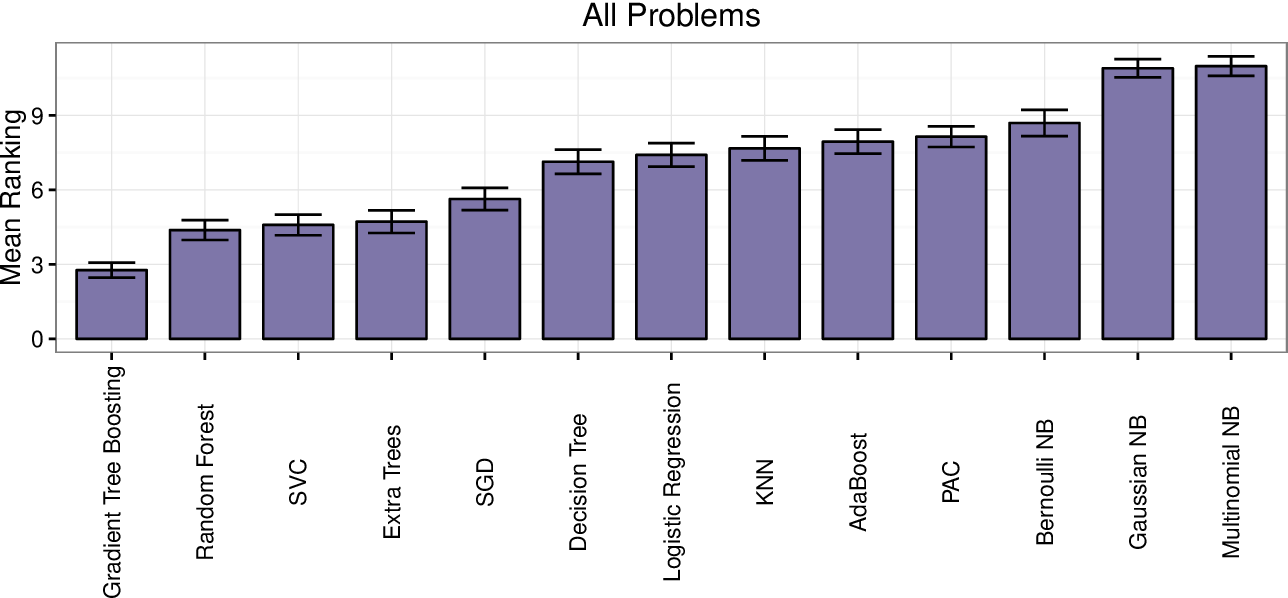
\includegraphics[width=0.8\textwidth]{Images/avarageRankingComparison.png}
    \caption[Durchschnittliche Platzierung der ML Algorithmen über allen Daten]{Durchschnittliche Platzierung der ML Algorithmen über allen Daten (Quelle \cite[Abbildung 1]{Olson2018})}
    \label{fig:avarage_ranking_comparison}
\end{figure}
\begin{figure}[H]
    \centering
    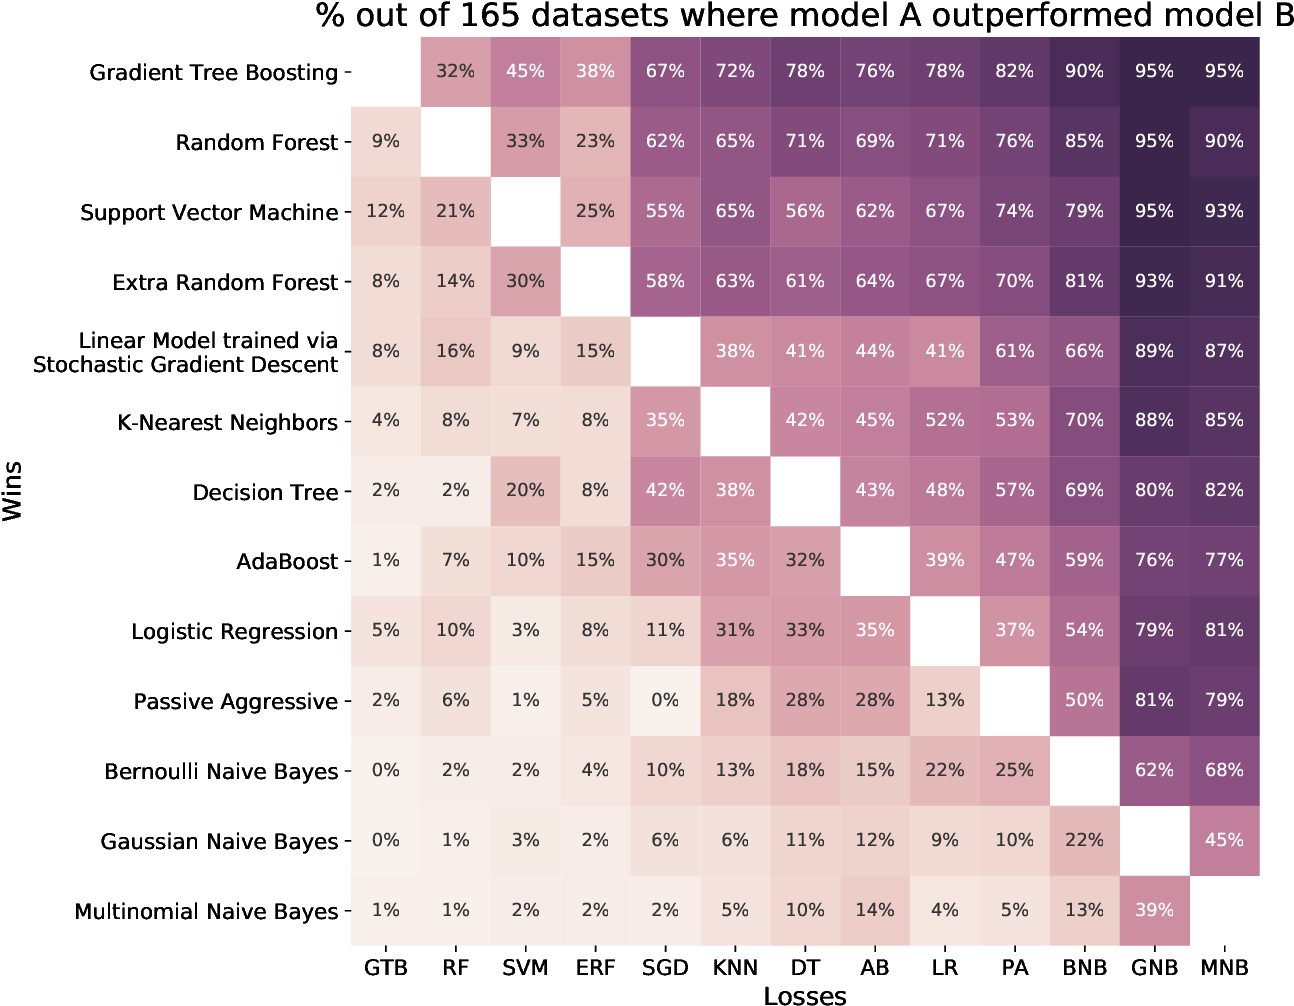
\includegraphics[width=0.75\textwidth]{Images/heat_map_comparison.png}
    \caption[Heatmap zum 1 zu 1 Vergleich der Algorithmen]{Die Abbildung  zeigt eine Heatmap, welche den Prozentsatz der 165 Datensätze darstellt, bei denen ein Algorithmus in Bezug auf die beste Genauigkeit auf einem Problem einen anderen übertrifft. Zwei Algorithmen sind als gleichwertig angesehen werden, wenn ihre Genauigkeit innerhalb von 1\% voneinander liegt. (Quelle \cite[Abbildung 2]{Olson2018})}
    \label{fig:heat_map_comparisom}
\end{figure}

\subsection{Interpretation der Ergebnisse}
\subsubsection{Bedeutung für AdaBoost und GBT}
Die Ergebnisse dieser Studie decken sich mit dem Leistungsvergleich aus Kapitel \ref{sec:performance_comparison}. Die Leistungsstärke von GBT wird verdeutlicht und unterstreicht seine Eignung für unterschiedlichste Probleme. Auch wenn AdaBoost vergleichsweise mittelmäßig abschneidet, ist das trotzdem eine beachtliche Leistung. Gerade für Datenstrukturen, die weniger komplex sind oder eine schnellere Trainingszeit benötigen, sollt man AdaBoost nicht außer Acht lassen.

\subsubsection{Empfehlungen für die Praxis}
Auch wenn GBT in den Tests am besten abgeschnitten hat, ist es keines Falls ratsam zu versuchen alle Probleme ausschließlich mit diesem Algorithmus zu lösen. Wie in allen Bereichen des Machine Learnings wird es nie einen Algorithmus der in allen Bereichen immer am besten abschneidet. Olson betont in seiner Studie besonders, dass die Wahl der Hyperparameter eine signifikante Rolle spielt bis hin zu Leistungsunterschieden von über 50\%. Jedes Problem muss einzeln betrachtet werden und durch feiner Abstimmung der Hyperparameter kann ein für den Einzelfall bestes Modell gefunden werden.